\section[Overall Description]{\hyperlink{toc}{Overall Description}}
\label{sec:overallDescription}
\subsection[Product Perspective]{\hyperlink{toc}{Product Perspective}}
	Thanks to the general introduction and the scope definition from the previous sections, we are now able to look at our system first from the outside and then from the inside. To deal with this description we are going to see the external interfaces the system has to interact with and then the definition of the model in order to have a feasible structure with them; at the end of the section \textbf{state diagrams} are used to emphasize the dynamic behavior of the most critical classes identified for the model.
	\subsubsection[System Interfaces]{\hyperlink{toc}{System Interfaces}}
		\label{sec:systemInterfaces}
		In this section we are going to deal with the interfaces that SafeStreets needs to \emph{use} in order to provide its functionalities. The definition of SafeStreet's interfaces to the external world, instead, will be described in the further related section (\ref{sec:externalInterfaceRequirements}), while precise details are given in the Design Document \cite{DD}.\\
	
		To accomplish the \hyperref[sec:goals]{\textbf{goals}} stated in the introduction the application interfaces with three main external systems as reported in the following picture (\autoref{fig:systemInterfaces}).  
		\vspace{0,3cm}
		
		\begin{figure}[h]
			\centering
			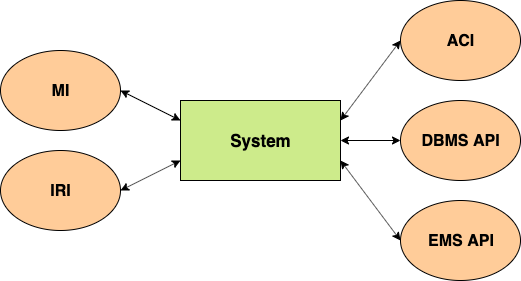
\includegraphics[scale=0.5]{externalInterfaces.png}
			\caption{\label{fig:systemInterfaces}System Interfaces}
		\end{figure}
		
		Two different kinds of interface are distinguished in the picture above:
		\begin{itemize}
			\item \textbf{Left hand side:} interfaces that provide functions for the system to perform internal algorithmic operations. In particular:
			\begin{itemize}
				\item \textsc{IRI} is used to process the pictures received from a violation. Whenever an infraction is reported, the application needs to retrieve the plate's number of the violation in order to be stored and notified to the authority. The image recognition algorithm "has always the last word": it uses the information provided by the user to help the recognition and, in all the cases a plate number will be found, it will be considered correct in the stored information and thus notifiable. Hence, whenever the algorithm does not recognize any plate number the entire notification will be discarded.
			
				\item \textsc{MI} is used to process the map issues. This interface provides three services fundamental for the application: the first is used to retrieve the exact street where a reported violation has occurred (using its GPS position), the second allows to find the best path between two position specified by the customer, while the third one offers the system a way to highlight a map with different colors when it provides to the functions a list of streets and their related colors. We will describe precisely in further sections how the street retrieval is used in the notification service while the map highlight in the safety one.
			\end{itemize}
			
			\item \textbf{Right hand side:} considers all the interfaces that involve an interaction with the authority. This means that this global interface manages both the accidents provided by the authorities and their PEC addresses: a publishing system will be needed to allow the authorities to publish their accidents in order to provide a way to retrieve them by the system. This interface allows also to possess all the information related to the PEC addresses of each authority the application has to manage.
			
		\end{itemize}
	
	\subsubsection[Model Structure]{\hyperlink{toc}{Model Structure}}
	The static analysis now continues to define the internal structure of the system, in particular with a high-level class diagram (\autoref{fig:classDiagram}) that considers the most important objects and their relations in order to achieve the functionalities described by the \hyperref[sec:goals]{\textbf{goals}}.\\
	
	The main objects in the UML class diagram are:
	\begin{itemize}
		\item \textbf{Customer:} the system has to track two types of clients. The distinction, in fact, is fundamental to recognize the municipality providing accident's data but also to give a different level of visibility to the information asked by a request. This class keeps track of the information related to the login (username and password).
		
		\item \textbf{User:} identifies a citizen with all the data he provides in its registration. Users are the clients of the application that report violations and mine the data related both to the frequency of parking violations and the most dangerous vehicles or to the safety of an area and its related suggested intervention.
		
		\item \textbf{Authority:} identifies both the authority/municipality with all the data related to its recognition. Authorities are the clients of the application that gets notified of the reported violations, but they also: mine for infractions and safety information and provide data about the accidents (crossed by the system).
		
		\item \textbf{Violation:} represents a general traffic violation. This class is thought to be used in a future extension of the system in case more violations are going to be considered.
		
		\item \textbf{ParkingViolation:} is the result of a notification provided by a user. In this way the application considers all the possible information that is filled whenever an infraction is reported. As we see in the UML diagram the class contains: multiple images for an improved help to both the image recognition algorithm and the authorities; the position retrieved by the GPS (used to find the name of the street); the type of the vehicle; the plate's number, date and time. The type of the violation, selected by the users will be determined considering one of the possible extending classes: \textbf{DoubleParking, DisabledZone, NoParkingZone, BikeLaneParking...} The relation with the safety class helps to highlight how \emph{safety} is determined as it will be precisely described in further sections \ref{sec:stateDiagrams} and \ref{sec:safetyFunction}.
		
		\item \textbf{Accident:} will be used to store the data received by the municipality by characterizing each accident as: \textbf{BikeCrash, MotorcycleCrash, CarCrash, ParkingHit...} The relation with the safety class helps to highlight how \emph{safety} is determined as it will be precisely described in further sections \ref{sec:stateDiagrams} and \ref{sec:safetyFunction}.
		
		\item \textbf{Position:} stores the coordinates obtained by the GPS of where the parking violation occurred. The position of each infraction will be used to retrieve the street thanks to the functionalities provided by the MI.
		
		\item \textbf{Street:} is one of the most important objects to be managed. Each recognized street will be added to the system to achieve its basic and advanced functionalities. As we see is one of the classes with the most relations, in fact: it defines the city and the path, it is queried by the mining and safety requests and has a possible suggestion associated in case it is considered unsafe. The relation with the safety class determines the one of the street.
		
		\item \textbf{City:} represents the entire area that is governed by a municipality. Also this class is important to be considered as a filter in the functionalities of the system but also for the requests.
		
		\item \textbf{Path:} represents the last way in which a filter about an area can be performed. This option is mainly thought for the advanced function about retrieving the most unsafe streets in the selected path.
		
		\item \textbf{Vehicle:} vehicles are considered in order to define the feasible types which have plates and thus that can be reported in a violation. Some examples of classes are: \textbf{Truck, Car, Motorcycle...}
		
		\item \textbf{Request:} is the general class representing the interaction of a user with the system whenever mining, safety or suggestion is asked by the customer. In order to answer with the correct data it will be important to retrieve the user who sends the request and provide it to him with the correct visibility.
		
		\item \textbf{BasicRequest:} is the request that deals with the basic functionality. It is extended in fact with the three different requests that can be performed by a customer: the two related to the mining service (\textbf{MostViolationsRequest} and \textbf{DangerousVehiclesRequest}), and the one that provides a different level of visibility to the authority (\textbf{FindReportsRequest}).
		
		\item \textbf{AdvancedRequest:} is the request that deals with the advanced functionality. It is extended in fact by the different requests that can be performed by a customer: \textbf{UnsafeStreetsRequest} and \textbf{InterventionRequest.}
		
		\item \textbf{PossibleIntervention:} represents a possible intervention suggested for a precise street. The relation with the safety class helps to highlight how \emph{safety} is determined as it will be precisely described in further sections \ref{sec:stateDiagrams} and \ref{sec:safetyFunction}.
		
		\item \textbf{Safety:} is a support class used to highlight the relations between the objects that determine whether a street is \textbf{safe} or \textbf{unsafe}.
	\end{itemize}
	
	\begin{figure}[h!]
		\centering
		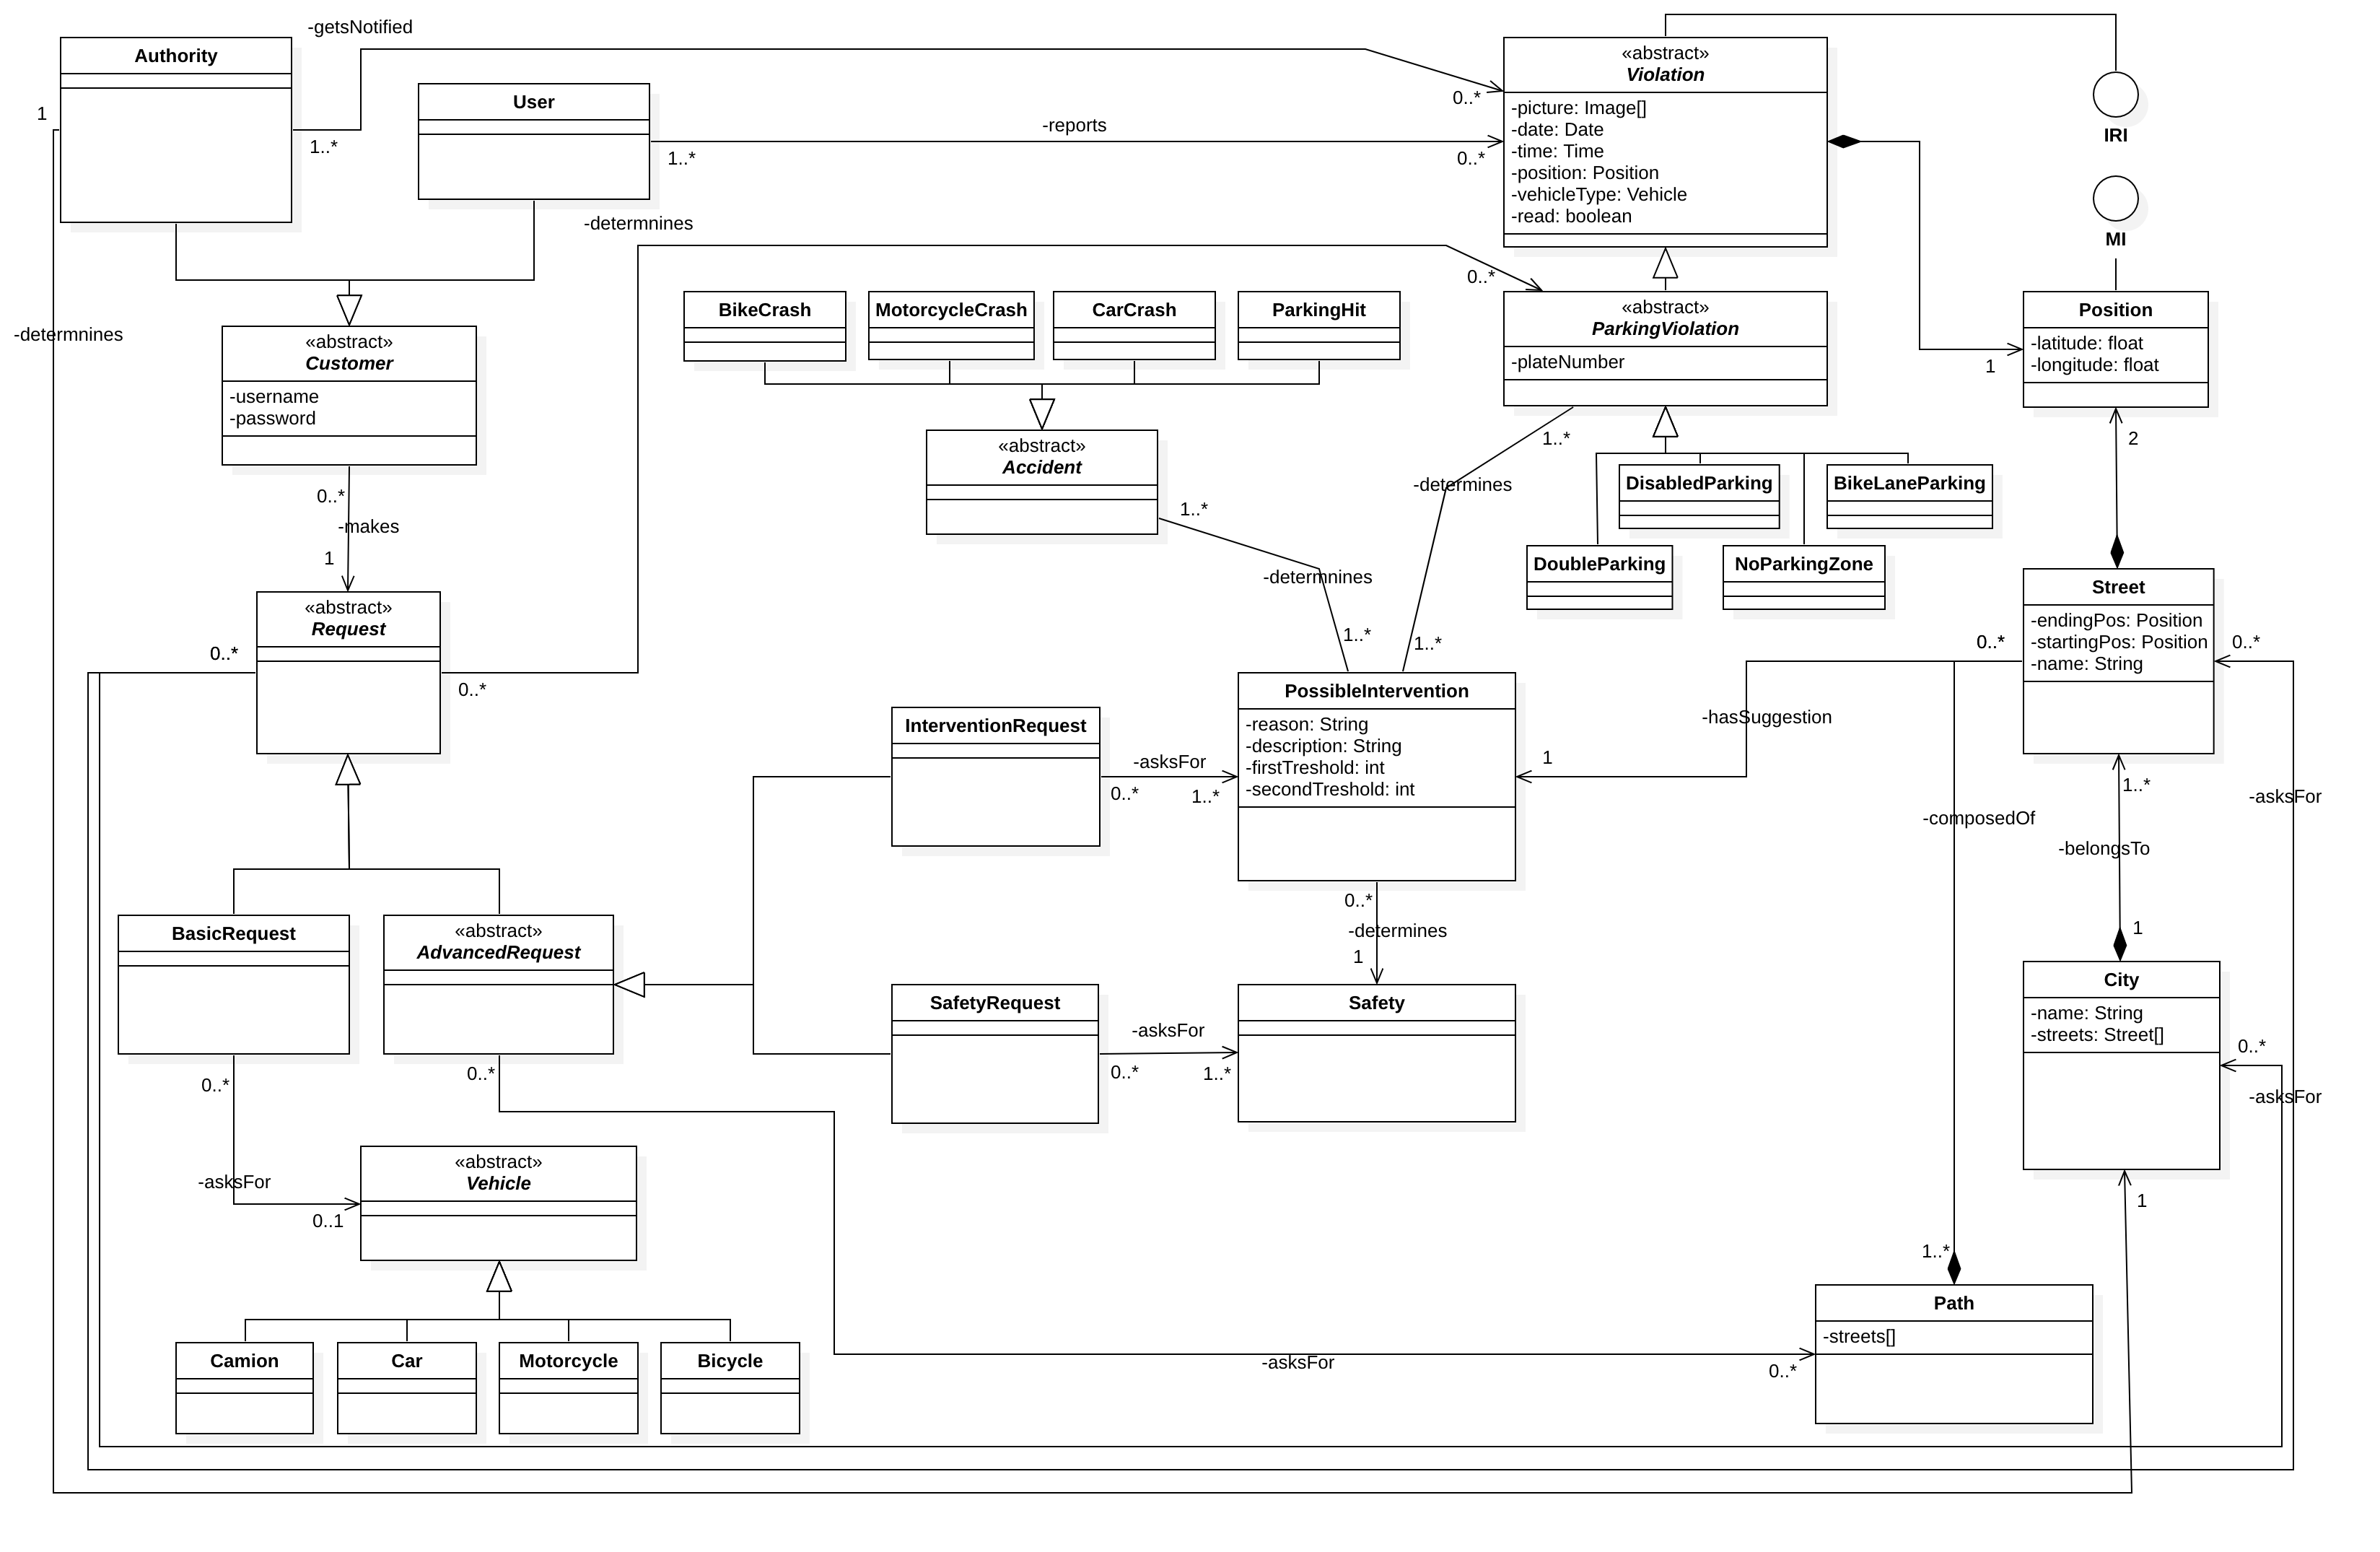
\includegraphics[width=\paperwidth - 1cm, angle=90]{/diagrams/classDiagramModel.png}
		\caption{\label{fig:classDiagram}High-level model structure}
	\end{figure}

	\FloatBarrier
	
	\subsubsection[State Diagrams]{\hyperlink{toc}{State Diagrams}}
	\label{sec:stateDiagrams}
		Considering now the main functionalities of the system, it is important to highlight the events that make its objects change their state. State diagrams are used to describe the most critical aspects of the objects previously described in the UML class diagram (\autoref{fig:classDiagram}).
		
		\paragraph{Notification}
			Starting with the report of a violation it is important to remember that each infraction will be refused by the system i.i.f no plate is found by the image recognition algorithm. The diagram (\autoref{fig:notifyState}) starts when a notification is received in the \textit{unprocessed} state. First the system needs to use the functionalities provided by the IRI in order to find the plate of the vehicle. If no plate number is found, the notification is \textit{rejected} and the diagram ends, otherwise the \textit{accepted} violation needs now to use the MI functionalities to retrieve the street where the infraction occurred. All the information about the violation is now known in the \textit{accepted} state, before storing and notifying it, the application has to look for duplicates checking in its stored data for a violation with the same: plate number, street, date and time, type of vehicle and type of violation. If a \textit{duplicate is found} the notification is still rejected by the system, otherwise it is stored and then notified to the related authority. The notification diagrams ends with the violation marked as \textbf{unread} for the authority that will be able, once logged in the system, to retrieve all the violations that occurred in its territory.
			
			\vspace{0.3cm}
			\begin{figure}[h]
				\centering
				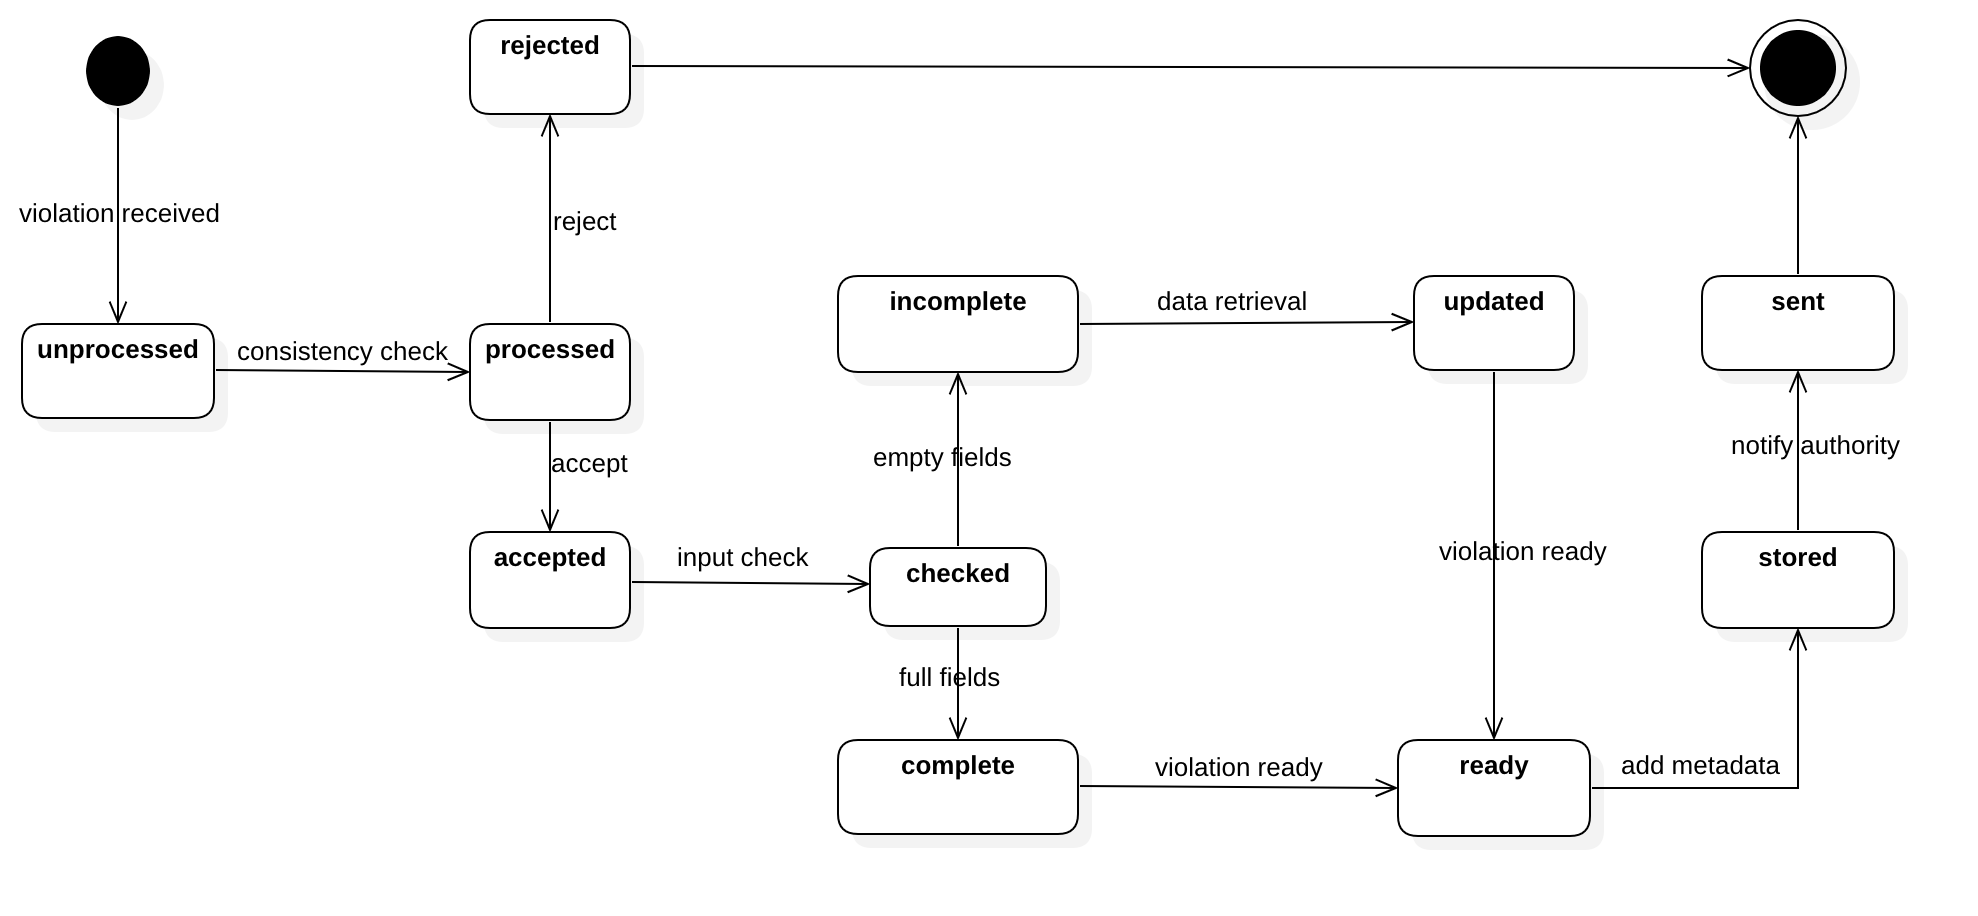
\includegraphics[scale=0.19]{/diagrams/state/notify.png}
				\caption{\label{fig:notifyState}Notification state diagram}
			\end{figure}
		
		\paragraph{Request}
			Information retrieval is another critical functionality that needs a state diagram to define how the information to be mined is provided with different levels of visibility depending on the role of the customer. The diagram (\autoref{fig:requestState}) considers in fact the process of how the query obtained by a request will be managed in order to avoid providing secret data to the users. Whenever a request is received the relative query will be retrieved in the \textit{unprocessed} state and then executed in the \textit{processed} one. A check is now needed in order to understand the kind of customer from which the request is coming. If the query comes from a customer who could perform it the data is \textit{accepted} and sent back to the inquirer, otherwise it is \textit{rejected} and the diagram ends.
			
			\vspace{0.3cm}
			\begin{figure}[h]
				\centering
				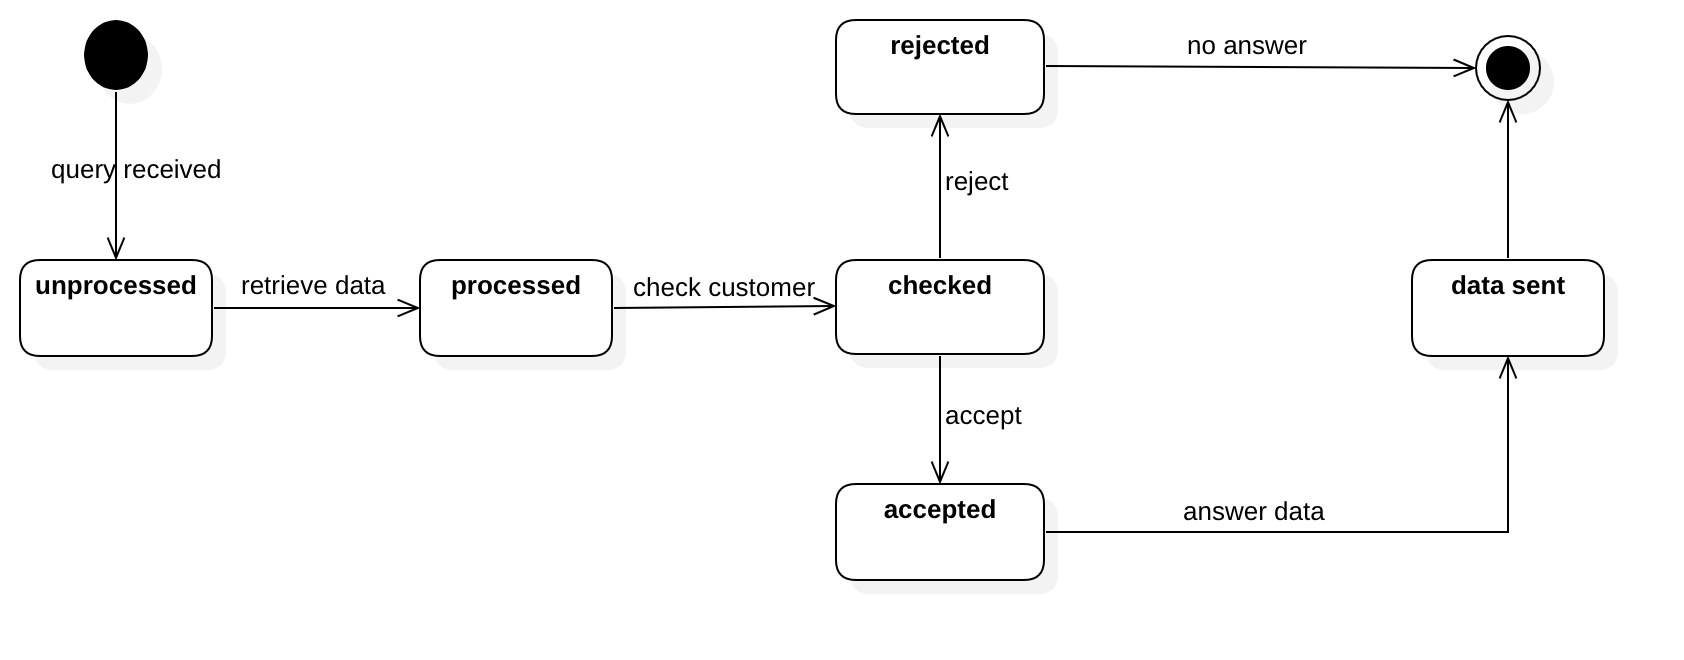
\includegraphics[scale=0.21]{/diagrams/state/request.png}
				\caption{\label{fig:requestState}Request for data state diagram}
			\end{figure}
		
		\paragraph{Safety}
			The last state diagram is used to highlight how the system is able to determine the safety of a street and update its state whenever new violations occur or new accidents data is provided by the municipality. The diagram (\autoref{fig:safetyState}) shows how the safety of a street evolves in the time. The system, each day, does two checks related to all the parking violations and accidents that occurred in a certain street in the previous 30 days. Two tresholds are defined to make the \textit{safe} state trigger: one is related to each \textbf{Possible Intervention} the other to the sum of all \textbf{Violations} and \textbf{Accidents}. It is enough that one treshold for a possible intervention \textbf{or} that the sum treshold is exceeded in order to reach the \textit{unsafe[RED]} state; the opposite happens for reaching the \textit{safe[GREEN]} one. In the section \ref{sec:safetyFunction} all details are provided to understand how this counting works, for now it is important to understand that thanks to it the safety of each street can be updated daily.
			
			\vspace{0.3cm}
			\begin{figure}[h]
				\centering
				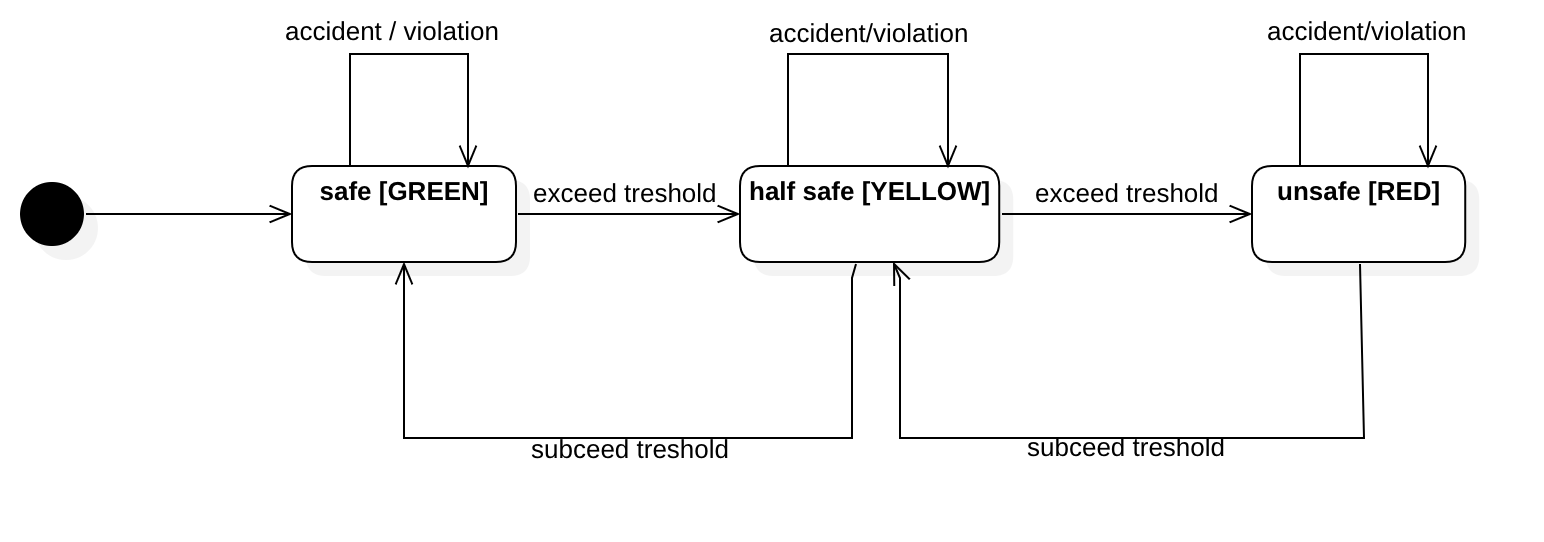
\includegraphics[scale=0.3]{/diagrams/state/safety.png}
				\caption{\label{fig:safetyState}Area safety state diagram}
			\end{figure}   

\subsection[Product Functions]{\hyperlink{toc}{Product Functions}}
	\label{sec:productFunctions}
	SafeStreet is a crowd-sourced application that intends to provide users with the possibility to notify authorities when parking violations occur. This has to be considered the main product function of the system because of its importance to obtain \textbf{crowdsourcing}. The information provided by users is what SafeStreet focuses on and what makes it able to provide services about the violations in a particular area. Thanks to mining and crossing processes, the system can retrieve filtered data about frequency, safety and suggestions for possible interventions in unsafe streets. As the subsection is structured, the product functions will be precisely described following the same order of how we have just shallowly presented: first the \textbf{notification} function then the \textbf{mining} one and in the end \textbf{safety}. \\
	
	Before starting with the description it is important to highlight that in order to benefit of SafeStreets functionalities the customer \textbf{must} be logged in the system as he can be recognized.
	
	\subsubsection[Notification Function]{\hyperlink{toc}{Notification Function}}
		\label{sec:notificationFunction}
		Users are allowed to notify authorities thanks to SafeStreets: the notification process takes place entirely inside the application. It starts when the user reports a violation and ends when the authority has the notification marked as unread in his interface (hence in the system too). Each user can report a violation as soon as he spots it, this means he is not allowed to notify it later; in this way we reduce the number of possible incorrect notifications as we have assumed that the \emph{date} and \emph{time} are automatically added by the application as well as the position, always retrieved because a user \textbf{must} enable his GPS before reporting any violation.\\
		
		The notification functionality is provided to the user by an interface that allows him to insert all the information needed to report a violation. The fields a user fills are reported here with a label that describes if they are mandatory or not.
		
		\begin{itemize}
			\item \textbf{Pictures}\texttt{[MANDATORY]:} users must provide at least one picture of the violation in order to report it. The pictures are taken \textbf{inside} the application where a functionality allows to select one or more of them; in this way we are sure that every image that has been received is authentic. Having always a picture it is possible to run the image recognition algorithm to understand the plate's number, in fact it is important to remark that whenever a number is not retrieved the entire violation will be discarded. Thanks to the option of inserting multiple images we provide a larger number of possibilities to recognize the plate; these pictures can be also very useful for the authorities that may decide in this way on which of the violations to take action first.
			
			\item \textbf{Position}\texttt{[MANDATORY]:} this field is marked as mandatory because, as we have previously said, the position will be retrieved by the GPS of the reporting device. The application does not allow a user to report a violation if its GPS service is not enabled, in this way, if a user is trying to report an infraction without the GPS, he will be forced to switch it on in order to complete the notification.
			
			\item \textbf{Type of Violation}\texttt{[MANDATORY]:} users need to give additional information providing also the type of the violation they are reporting. This kind of data is used as a filter in the mining functionalities and it can be a very useful knowledge to both users and authorities.
			
			\item \textbf{Type of Vehicle}\texttt{[MANDATORY]:} users must provide also this information in order to complete the notification. It is another filter in the mining functionalities.
			
			\item \textbf{Plate}\texttt{[OPTIONAL]:} this field is thought to give additional information to the functionalities provided by the IRI in order to recognize the plate of the reported vehicle. As we have already said it is the image recognition algorithm who has the last word when deciding whether to discard or not a violation: if he recognizes a number, also thanks to this information, the notification will be considered, otherwise it will not be.
		\end{itemize}
	
		Once the notification is received the system first tries to retrieve the plate of the reported vehicle. If the plate's number is found it means that the violation is valid and the check for duplicates can be carried out. If no duplicate is found, the violation is ready to be stored in the system and thus notified to the authority. The \textbf{notification} works as follows: each violation that has been accepted is stored as \textbf{unread} for the authority that governs the territory that contains its street, in this way, when the authority enters the system it will be able to see all the notifications that have been reported. Once checked by the authorities the notifications will be marked as \textbf{read} and removed from the \emph{Check Unread Reports} functionality. Even if a notification for an authority that is not registered to the system yet is received by the system, it will be stored and marked as unread in order not to loose this information.

	\subsubsection[Statistics Function]{\hyperlink{toc}{Mining Function}}
		Data mining is used to retrieve the information about the stored data and provide the customers different ways to filter it. Thanks to the details of each infraction, in fact, the system is able to offer this service both to users and authorities. \\
		
		Two functionalities are offered to customers thanks to the mining process: 
		
		\begin{itemize}
			\item \textbf{Highest Number of Violations:} returns an ordered list of the streets where the highest numbers of violations occur.
			\item \textbf{Most Dangerous Vehicles:} returns an ordered list of the types of vehicles that make the highest number of violations.
		\end{itemize}
		
		 Both these functionalities but also the one allowed only to the authorities (\emph{Find Reports}) can be filtered with some of the the filters listed below.
			
		\begin{itemize}
			\item \textbf{Area:} there are three levels of filters defined in the area one. The widest is called \textbf{everywhere} and returns the information generally all over Italy, the second is called \textbf{city} and considers all the streets contained in the specified city, and the most specific one considers just a single \textbf{street}.
			
			\item \textbf{Date:} this filter is allowed only to authorities in the \emph{find reports} functionality, in this way they are able to retrieve the violations in a more detailed search.
			
			\item \textbf{Time:} customers are able to filter by choosing a time lapse in which they are interested in. 
			
			\item \textbf{Type of vehicles:} the system stores in each notification the type of the vehicle that committed the violation. In this way this data can be filtered choosing one of the types: \textbf{trucks, cars, motorcycles...}
			
			\item \textbf{Type of violation:} thanks to the information about the type of the violation (provided by the user) the application allows also to filter by type. We can think of this  mainly filter for the authorities who will look for the highest type of vehicles that commit a violation in a street in order to take action; however this filter is also allowed to users who may be interested in this kind of data too.
		\end{itemize}
	
		Each functionality considers only the filters that are needed to achieve its mining process. As we see in the interfaces (section \ref{sec:userInterfaces}) and in the use case diagrams (section \ref{sec:useCases}) just some of the listed filters are allowed to be selected. \\
		
		It is important to highlight that SafeStreets provides information to customers with different levels of visibility depending on their role. To accomplish this distinction the system provides the authorities an additional functionality that allows them to retrieve the information in the highest level of detail possible. \emph{Highest Number of Violations} and \emph{Most Dangerous Vehicles} are in fact statistical functionalities that are not meant to be provided differently depending on the user that is requiring them. Moreover the \textbf{Find Reports} functionality is able to give the authorities a way to retrieve each violation in detail as it is stored in the system. This functionality is the one that contains the highest number of filters as it can provide a specific way to retrieve the violations of interest to the authorities. 

	\subsubsection[Safety Function]{\hyperlink{toc}{Safety Function}}
		\label{sec:safetyFunction}
		SafeStreets is able to process the information provided by the municipality about the accidents that occur in a territory. Thanks to this additional data the system can cross it with its stored one and determine the \textbf{safety} of each street as we now precisely describe. Whenever a municipality is not able to provide the information about the accidents to SafeStreets the safety can be still determined thanks to the mathematical model further defined that will just use the information stored about the violations. \\
		
		The system dynamically changes the safety of a streets thanks to two different kinds of treshold defined for each street:
		
		\begin{enumerate}
			\item \textbf{Intervention Treshold:} each intervention has a "personal" treshold that once exceeded determines a street to be unsafe. Every type of accident or violation is related to one or more intervention so that, once they occur in a street they make increase the counter of each intervention. If one of the counters of the interventions for a street exceeds the treshold it means that the street has become \textbf{unsafe} and that the exceeded intervention should be taken into account as the suggestion to enhance the \textbf{safety} of the now dangerous street.
			
			\item \textbf{Sum Treshold:} another treshold is needed to consider also the accidents that are not related to any intervention but anyway determine a street to be \textbf{unsafe}. This treshold is based on the sum of the accidents and parking violations that occur in the street. If the sum exceeds the treshold it means that the street has become \textbf{unsafe} and the related possible intervention is the one whose counter is the nearest to the treshold.
		\end{enumerate}
	
		Hence the first of the two types of treshold that is exceeded in a street determines it to be unsafe.
		The safety of each street and then the related intervention is determined each day by the system with the stored information about the previous month. Thanks to the data retrieved by the \emph{crossing} process, SafeStreets is able to provide the following functionalities:
		
		 \begin{itemize}
		 	\item \textbf{Unsafe Streets:} thanks to the MI SafeStreets can use its services to retrieve the portion of an area and highlight its streets with two different colors to distinguish \emph{safe streets} colored in \textbf{GREEN} from \emph{unsafe streets} colored in \textbf{RED}. The map interface provides functions that require a set of streets and the colors to be highlighted with and returns the best positioned map with the respective colors. 
		 	
		 	\item \textbf{Urgent Interventions:} thanks to the tresholds we always at least one suggestion for a possible intervention whenever a street is considered to be unsafe. This functionality allows the customers to retrieve the possible interventions for the area in which they are interested in.
		 \end{itemize}
	 
	 	Both these functionalities in fact can be filtered in order to reduce the size of the interested area, the possible filters used in one or the other are: \textbf{city, path, street.}
		
\subsection[User Characteristics]{\hyperlink{toc}{User Characteristics}}
	\label{sec:userCharacteristics}
	SafeStreets has two different customers that are very important to distinguish in order to provide correctly the functionalities previously described in subsection \ref{sec:productFunctions}. In the entire document a general client is called \textbf{customer} and the distinction is made between:
	
	\begin{itemize}
		\item \textbf{USER}
			\begin{itemize}
				\item Always inserts correct data while registering.
				\item Always inserts correct data while reporting violations.
				\item Can not register with a username that corresponds to an existing PEC address.
				\item Must have a device to take pictures of a parking violation.
				\item Must enable the GPS of the device in order to report a violation.
				\item Can register to SafeStreets in order to be recognized as such.
				\item Must login to SafeStreets to benefit of its services.
				\item Can filter the mined data.
				\item Can retrieve the safety of a street.
				\item Can retrieve the suggestion for a possible intervention of an unsafe street.
			\end{itemize}
		\item \textbf{AUTHORITY/MUNICIPALITY}
			\begin{itemize}
				\item Are supposed to be in Italy.
				\item Always inserts correct data while registering.
				\item Knows the PEC address of the territory they manage.
				\item Provides correct information about accidents.
				\item Can register to SafeStreets in order to be recognized as such with their PEC address.
				\item Must login to SafeStreets to benefit of its services.
				\item Can search for detailed violations.
				\item Can filter the mined data.
				\item Can provide information about the accidents that occur in its territory.
				\item Can retrieve the safety of a street.
				\item Can retrieve the suggestion for a possible intervention of an unsafe street.
			\end{itemize}
	\end{itemize}
	
\subsection[Domain Assumptions]{\hyperlink{toc}{Domain Assumptions}}
	\label{sec:domainAssumptions}
	Domain assumptions are used to define clearly the world in which SafeStreets is involved. Thanks to them we are able to add constraints that define the bounds of the environment. It is first important to give the description of one of these assumption to precise why we decided to consider it. The fact that \emph{The system is allowed to work in Italy} is used to deal with the recognition of the authorities. It is very important in fact to be sure of the identity of each customer in order to manage the security of the stored data, problems relative to the law and simplify the description with only the correct level of details. Thanks to this assumption in fact we can consider that every authority knows its PEC address and thus use this existing technology to define the recognition process. \\
	
	We assume that these assumptions hold true in the domain of the system:
		
	\begin{enumerate}[label=\textbf{DA\arabic*}]
		\item \label{dom:correctRegistration} Customers always insert correct data while registering to SafeStreets.
		\item \label{dom:correctViolation} Users always insert correct data while reporting violations to SafeStreets.
		\item \label{dom:pecKnown} The association between cities and PEC is well-known by SafeStreets.
		\item \label{dom:uniquePec} PEC addresses are unique.
		\item \label{dom:specialCharacters} Special characters are all the characters that are not letters nor numbers.
		\item \label{dom:correctDateTime} Date and time on the devices on which SafeStreets runs are always correct.
		\item \label{dom:gpsAccuracy} The GPS module of the devices on which SafeStreets runs always works correctly and has an accuracy of 2 meters.
		\item \label{dom:correctCamera} The camera module of the devices on which SafeStreets runs always works correctly.
		\item \label{dom:correctInternet} Internet connection works always without errors.
		\item \label{dom:italy} The system is assumed to work in Italy.
		\item \label{dom:italyMaps} Maps of Italy are well known, complete and up to date.
		\item \label{dom:nonameStreets} There are no streets without a name.
		\item \label{dom:noMaliciousPlates} No one physically and maliciously replaces license plates.
		\item \label{dom:nosameCities} There are no cities with the same name in a given region.
		\item \label{dom:nosameStreets} In a city there are not streets with the same name.
		\item \label{dom:streetCity} Every street belongs exactly to one city.
		\item \label{dom:correctAccidents} Accidents data provided by municipalities are always correct.
		\item \label{dom:nomultipleViolations} No multiple violations of the same vehicle occur in the same place at the same time.
	\end{enumerate} 
	
\subsection[The World and the Machine]{\hyperlink{toc}{The World and the Machine}}
	\label{sec:worldMachine}
	Thanks to the constraints on the domain of interest for the system (section \ref{sec:domainAssumptions}), we are now able to describe SafeStreets with the \textit{World and the Machine} approach that allows to underline the most important phenomena that are present in the problem we are dealing with. The machine represents the system do be developed while the world (a.k.a environment) is the portion of the real world affected by the machine.\\
	
	Thanks to this distinction we highlight in the next picture (\autoref{fig:worldAndMachine}) the main phenomena of our problem: the ones in the world affect the world only, the ones in the machine affect the machine only and the ones in between affect both the world and the machine. This figure can be also used to start guessing the requirements (section \ref{sec:specificRequirements}) of our system as they can be defined as: \textit{prescriptive assertions formulated in terms of shared phenomena.}
	\vspace{1cm} 
	
	\begin{figure}[h]
		\centering
		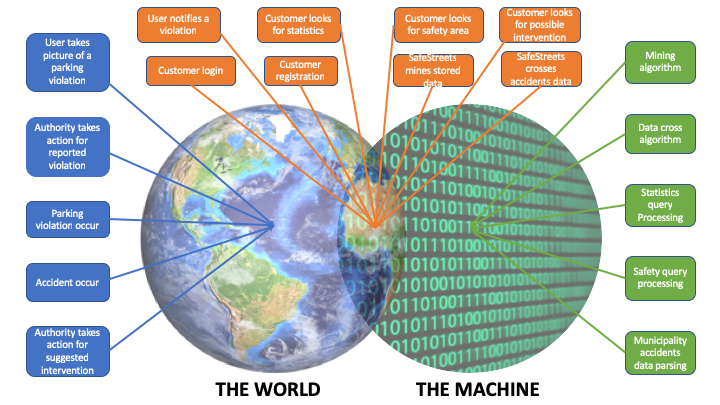
\includegraphics[scale=0.82, angle=90]{WorldAndMachine.png}
		\caption{\label{fig:worldAndMachine}The World and the Machine}
	\end{figure}
 	 